%%%%%%%%%%%%%%%%%%%%%%%%%%%%%%%%%%%%%%%%%%%%%%%%%%%%%%%
%                File: OpEx_temp.tex                  %
%             Created: 2 September 2009               %
%                Updated: 15 May 2015                 %
%                                                     %
%           LaTeX template file for use with          %
%           OSA's journals Optics Express,            %
%             Biomedical Optics Express,              %
%            and Optical Materials Express            %
%                                                     %
%  send comments to Theresa Miller, tmiller@osa.org   %
%                                                     %
% This file requires style file, opex3.sty, under     %
%              the LaTeX article class                %
%                                                     %
%   \documentclass[10pt,letterpaper]{article}         %
%   \usepackage{opex3}                                %
%                                                     %
%                                                     %
%       (c) 2015 Optical Society of America           %
%%%%%%%%%%%%%%%%%%%%%%%%%%%%%%%%%%%%%%%%%%%%%%%%%%%%%%%

%%%%%%%%%%%%%%%%%%%%%%% preamble %%%%%%%%%%%%%%%%%%%%%%%%%%%
\documentclass[10pt,letterpaper]{article}
\usepackage{opex3}
\usepackage{color}
\usepackage[latin9]{inputenc}
\usepackage{amsmath}
\usepackage{graphicx}%
\usepackage{float}
\usepackage{amsfonts}%
\usepackage{amssymb}
\usepackage{braket}
\usepackage{bm}
\newcommand{\mb}[1]{\bm{#1}}
\usepackage[T1]{fontenc}

%%%%%%%%%%%%%%%%%%%%%%% begin %%%%%%%%%%%%%%%%%%%%%%%%%%%%%%
\begin{document}

%%%%%%%%%%%%%%%%%% title page information %%%%%%%%%%%%%%%%%%
\title{Simple template for authors submitting to OSA Express Journals}

\author{Petar Tzenov$^{1,*}$, Christian Jirauschek$^1$ and David Burghoff$^{2}$}

\address{$^1$ Institute for Nanoelectronics, Technische Universit\''at M\''unchen, D-80333 Munich, Germany}
\address{$^2$ Somewhere in MIT, US}

\email{$^*$petar.tzenov@tum.de} %% email address is required

% \homepage{http:...} %% author's URL, if desired

%%%%%%%%%%%%%%%%%%% abstract and OCIS codes %%%%%%%%%%%%%%%%
%% [use \begin{abstract*}...\end{abstract*} if exempt from copyright]

\begin{abstract}
A simple template with few examples is provided for preparing \textit{Optics Express}, \textit{Biomedical Optics Express}, and \textit{Optical Materials Express} manuscripts in \LaTeX. For complete instructions, refer to \texttt{OpEx\_temp.txt}. The Express journal simple and extended templates are also available on \url{http://www.overleaf.com/gallery/tagged/osa}. OSA encourages the use of this free online collaborative tool for writing your OSA article.
\end{abstract}

\ocis{(000.0000) General.} % REPLACE WITH CORRECT OCIS CODES FOR YOUR ARTICLE, MINIMUM OF TWO; Avoid using the OCIS codes for “General” or “General science” whenever possible.

%%%%%%%%%%%%%%%%%%%%%%% References %%%%%%%%%%%%%%%%%%%%%%%%%
\begin{thebibliography}{99}

\bibitem{gallo99} K. Gallo and G. Assanto, ``All-optical diode based on second-harmonic generation in an asymmetric waveguide,'' \josab {\bf 16}(2), 267--269 (1999).

\end{thebibliography}

%%%%%%%%%%%%%%%%%%%%%%%%%%  body  %%%%%%%%%%%%%%%%%%%%%%%%%%
\section{Outline}

\begin{enumerate}
	\item{Introduction} 
	\item{Theoretical model: 3lvl LO-phonon THz QCL. Periodic rate equations  generalization to quantum mechanical DM equations.}
	\item{Generalization to more than three levels. Case study: Highly coherent resonant LO-phonon THz frequency comb. Monte carlo simulations, TB approximation. Regimes of validity of our model. } 
	\item{Comparrison between simulation and experimental data}
	\item{Conclusion}
\end{enumerate}

\section{Introduction}
\label{sec:intro}
Some words on the model, the neccessity its application and obtained results. Outline of the paper.
\section{Theoretical Model}

The Maxwell-Bloch (MB) equations are a semi-classical model describing the light-matter interaction in microscopic systems, where the coherent coupling between the optical field and the gain medium is modelled by density matrix, i.e. Bloch, equations, whereas the effect of the induced polarization onto the incident electric field, by the classical Maxwell's equations. This model is a generalization of the rate equations approach, which allows the inclusion of optical nonlinearities and coherence effects into electron transport simulations and thus incorporate the physics of four wave mixing and resonant tunneling into the system dynamics. In this paper, based on the previous work by many, we start by a derivation of the Maxwell-Bloch equations for a three level system with a single resonant-tunneling  and a single optical transition. Furthermore, we employ the rotating wave and slowly varying amplitude approximations to obtain a closed set of equations, describing the temporal evolution of the density matrix as well as the optical field. Lastly, we phenomenologically include into our density matrix equations the effect of nonradiative scattering mechanisms via the so called ``periodic rate equations approach''. Our model suffers from the limitation that it does not consider electron distribution in $\mathbf{k}-$space, which however we believe is not a significant drawback at low operating temperatures. In this form the equations comprise a full model for efficient long time simulations of light-matter interaction in laser systems. We believe that such simulations are vital for the investigation of the transient dynamics of complex multimode lasers, such as quantum cascade laser based THz frequency combs, understanding of which is very hard with analytical or steady state solutions alone. 
\begin{figure}[h!]
\centering
\includegraphics[scale=1]{img01.png}
\caption{Insert caption here} \label{fig:img01}
\end{figure}

Let us consider a simple three level resonant phonon QCL system as depicted in Fig. \ref{fig:img01}. In this configuration, there are four relevant laser levels $\Ket{1'}, \Ket{3}, \Ket{2} $ and $\Ket{1}$ which are the injector level, the upper and lower laser levels and the depopulation level, respectively. $\Ket{1'}$ couples to $\Ket{3}$ via the anticrossing energy $2\hbar\Omega_{1'3}$, whereas the upper and lower laser levels interact via the optical Rabi frequency $\Omega_L(t)= \mu_{32}E_z(t)/\hbar$, where $\mu_{32} = e \Bra{3}\hat{z} \Ket{2}$ is the dipole matrix element, $E_z(t)$ is the electric field component along the growth diraction $z$ and $e$ is the elementary charge. Lastly, we assume that the energy separation between $\Ket{1'}$ and $\Ket{3}$ is $\Delta_{1'3} = \hbar \epsilon$ and that between the upper and lower laser levels $\Delta_{32} = \hbar \omega_c$.
Following the standard derivation procedures of the MB equations we will employ a density matrix approach to describe the evolution of our statistical ensemble of electrons, coupled via a polarization term to a classical wave propagation equation. 
Within the density matrix formalism,  the equation of motion (EOM) that describes the evolution of the system is given by the von Neumann equation:
\begin{align}
 \label{eq:vonNeumann}
 i\hbar \frac{d \hat{\rho}}{dt} = [\hat{H};\hat{\rho}] ,
\end{align}
where $\hat{\rho}$ is the density operator, $\hat{H}$ the Hamiltonian of the system, and $[\cdot;\cdot]$ the usual quantum mechanical commutator. In general, $\hat{H}$ contains many different contributions corresponding to various physical mechanisms that determine the overall carrier transport in the system. These could be radiative transitions or coherent and incoherent scattering events such as resonant tunnelling for the former and LO phonon, electron-electron, interface roughness etc. for the latter. In principle, each scattering process enters Eq. (\ref{eq:vonNeumann}) as via its potential operator $\hat{V}$. If one was to include all relevant mechanisms into the equation, this will necessitate additional k-space discretization and the evaluation of the corresponding matrix equation into each point in space, time and transverse momentum. This requires tremendous numerical effort and renders such simulations impractical. We resolve this problem by treating only the coherent and radiative scattering mechanisms quantum mechanically, whereas all of the above enumerated incoherent processes will be treated semi-classically, i.e. via a rate equation approach. Furthermore, the rates for each separate scattering event are not chosen arbitrarily, but instead are calculated with our well established ensemble Monte Carlo simulation code.

When resonant tunneling transitions are modelled, one usually employs the so called tight-binding approximation, where the wave funcitons are calculated for a single isolated period, whereas the electron subbands in adjacent modules are simply translated in space and energy by the module length $L_p$. However, the true time evolution of the system is still governed by the full Hamiltonian, so we need to correct for the fact that we are using a tight-binding basis, by including the correct anticrossing, or coupling energies, between levels spanning a intermodule barrier. In our case these are the injector and upper laser level and the resonant-tunneling coupling energy is assumed to be $\hbar \Omega_{1'3}$. Finally in this tight-binding basis, one can write the von Neumann equaiton in matrix form as:
\begin{align}
 \label{eq:vonNeumannmatrix}
i \hbar \frac{d}{dt} \begin{pmatrix}
\rho_{1'1'}& \rho_{1'3} & \rho_{1'2} \\
\rho_{31'} & \rho_{33} & \rho_{32} \\ 
\rho_{21'} & \rho_{23} & \rho_{22}
\end{pmatrix}  = 
\left [ 
\begin{pmatrix} 
 \frac{\hbar \epsilon}{2} & \hbar\Omega_{1'3} & 0 \\
\hbar\Omega_{1'3}  & -\frac{\hbar	\epsilon}{2} &  \hbar\Omega_{L}(t) \\
0  &\hbar\Omega_{L}(t) & \frac{\hbar \epsilon}{2}-\hbar\omega_{c}   
\end{pmatrix} 
; 
\begin{pmatrix}
\rho_{1'1'}& \rho_{1'3} & \rho_{1'2} \\
\rho_{31'} & \rho_{33} & \rho_{32} \\ 
\rho_{21'} & \rho_{23} & \rho_{22}
\end{pmatrix}
\right ] , 
\end{align}
where $\rho_{i,j} = \Bra{i} \hat{\rho} \Ket{j}$ are the corresponding density matrix elements and we have set the zero energy at $E_0 = (E_{1'}+E_{3})/2 $. Notice that in Eq. (\ref{eq:vonNeumannmatrix}) we have omitted the time evolution related to the state $\Ket{1}$. This is due to the fact that the depopulation level, $\Ket{1}$, is effectively the injector level of the next period, which, as will be shown in Sec. \ref{subsec:periodicrate}, allows us to eliminate it from the model. Finally other scattering mechanisms due to spontaneous emission, LO-phonon scattering, electron-electron scattering etc., the so called collision terms, will be included in our model phenomenologically within a rate equation approach in the subsection that follows. 

Since the density matrix has the Hermitian property, Eq. (\ref{eq:vonNeumannmatrix}) boils down to a system of six coupled ordinary differential equations for the unknowns $\rho_{1'1'}, \rho_{33},\rho_{22},\rho_{1'3},\rho_{32} $ and $\rho_{1'2}$. Expanded, Eq. (\ref{eq:vonNeumannmatrix}) looks as:
\begin{align}
\frac{d \rho_{1'1'}}{d t} &= i\Omega_{1'3} (\rho_{1'3} - \rho_{31'}), \nonumber\\ 
\frac{d \rho_{33}}{d t}   &= i\Omega_{1'3} (\rho_{31'} - \rho_{1'3}) + i\frac{\mu_{32} E}{\hbar} (\rho_{32}-\rho_{23}),  \nonumber\\
\frac{d \rho_{22}}{d t}   &=- i\frac{\mu_{32} E}{\hbar} (\rho_{32}-\rho_{23}) , \nonumber\\
\frac{d \rho_{1'3}}{d t}  &= -i\epsilon\rho_{1'3} +i \Omega_{1'3}(\rho_{1'1'} - \rho_{33}) +i\frac{\mu_{32}E}{\hbar}\rho_{1'2}, \nonumber\\
\frac{d \rho_{32}}{d t}   &= -i\omega_{c}\rho_{32} +i \frac{\mu_{32}E}{\hbar}(\rho_{33}-\rho_{22}) -i\Omega_{1'3}\rho_{1'2} , \nonumber  \\
\frac{d \rho_{1'2}}{d t}  &= -i(\epsilon+\omega_c)\rho_{1'2} +i\frac{\mu_{32}E}{\hbar}\rho_{1'3} -i\Omega_{1'3}\rho_{32} . \label{eq:vonNeumannexpanded}
\end{align}
The essence of the Maxwell-Bloch equations is now in the couplig of the microscopic density matrix equations to the macroscopic Maxwell's equations. This is usually done via the incorporation of  polarization term in Maxwell's equations as the expectation value of the quantum mechanical dipole moment operator, i.e. :
\begin{equation} 
P_z = -N\Gamma Tr\{\hat\rho \hat\mu\} = -N\Gamma(\mu_{32}\rho_{32} + \mu_{23}\rho_{23}) =  -N\Gamma\mu_{32}(\rho_{32}+\rho_{23}) ,
\end{equation}
where $N$ is the average carrier density per unit volume and $\Gamma$ is the spatial overalp between the optical field  and the active region. The negative sign in the above expression is due to the fact that we have taken the dipole element as $e \Bra{3}\hat{z} \Ket{2}$ instead of$-e \Bra{3}\hat{z} \Ket{2}$. Assuming no free electric charges and also weak inhomogenities in the polarization field, we obtain the classical wave equation for  $E_z$:
\begin{equation}
(\partial^2_{x} -\frac{n^2}{c^2}\partial^2_t) E_z = \frac{1}{\epsilon_0 c^2}\partial^2_t P_z, 
\label{eq:fullwave}
\end{equation}
where $x$ denotes the propagation direction. Lastly, we have taken a constant background refractive index $n=\sqrt{\epsilon_r}$, which for GaAs systems is reported to be around $n = 3.6$.
\subsection{Periodic rate equations approach}
\label{subsec:periodicrate}
\begin{figure}[h!]
\centering
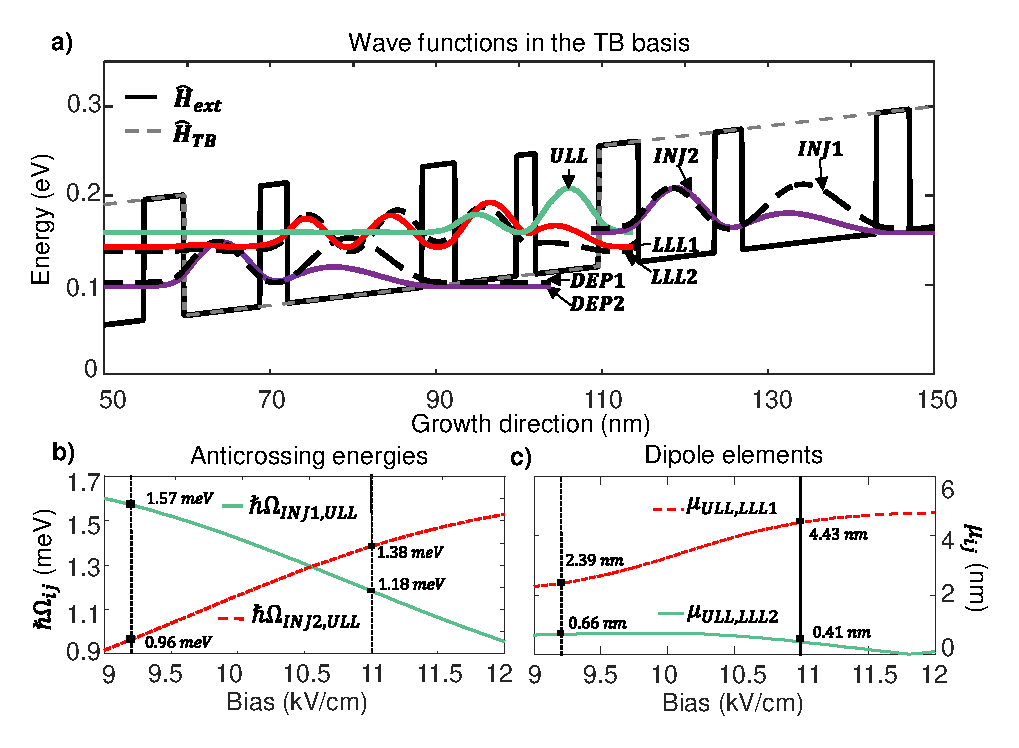
\includegraphics[scale=0.7]{img02} \caption{ Insert caption here}\label{fig:rate_equations}
\end{figure}
Let us consider the electron transport throught a ``source-transport channel-drain'' system , as depicted in Fig. \ref{fig:rate_equations}. Assume that electrons enter into the system via input current $I_{in}$, injected directly into the source. From there, take that the electrons scatter into one of $N$ channel levels, before they enter the drain and are consecuitively extracted out of the system in the form of output current $I_{out}$. We can write down the rate equations for this configuration as:
\begin{align}
& \frac{d n_S} {dt } = V^{-1}e^{-1}I_{in} +  \sum_{i=1}^{N} \tau_{iS}^{-1}n_i + \tau_{DS}^{-1} n_D - \left( \sum_{i=1}^N \tau_{Si}^{-1} + \tau_{SD}^{-1}\right) n_S, \nonumber \\
& \frac{d n_j} {dt } = \tau_{Sj}^{-1} n_S +   \sum_{i=1 , i\neq j}^{N} \tau_{ij}^{-1}n_i + \tau_{Dj}^{-1} n_D - \left(  \tau_{jS}^{-1}  + \sum_{i=1 , i\neq j}^N \tau_{ji}^{-1}  + \tau_{jD}^{-1}\right) n_j, \nonumber \\
& \frac{d n_D} {dt } =  -V^{-1}e^{-1}I_{out}  + \tau_{SD}^{-1} n_S +   \sum_{i=1}^{N} \tau_{iD}^{-1}n_i - \left(  \tau_{DS}^{-1}  + \sum_{i=1}^N \tau_{Di}^{-1}  \right) n_D, \nonumber
\end{align} 
where  $n_j$ denotes the carrier density (per unit volume) in level $j$ and $\tau_{ij}^{-1}$ the total outscattering rate from level $i$ to level $j$. Now, let us implement ``periodic'' boundary conditions to the above system, i.e. let us assume that every electron that enters the drain is immediately pumped back into the source. Then it follows that the carrier density $n_D \approx 0$ and that $I_{out} = I_{in}$. Using these assuptions, we can solve $dn_D/dt = 0$  for the current to get:
\begin{equation}
\label{eq:current}
I = Ve\left(\tau_{SD}^{-1} n_S +   \sum_{i=1}^{N} \tau_{iD}^{-1}n_i\right). 
\end{equation}
Using expression Eq. (\ref{eq:current}), and the assumption $n_D \approx 0$, we can rewrite the rate equations for our periodic system as:
\begin{align}
& \frac{d n_S} {dt } =  \sum_{i=1}^{N} \left( \tau_{iS}^{-1} + \tau_{iD}^{-1} \right) n_i  - \left( \sum_{i=1}^N \tau_{Si}^{-1} \right) n_S, \nonumber \\
& \frac{d n_j} {dt } = \tau_{Sj}^{-1} n_S +   \sum_{i=1 , i\neq j}^{N} \tau_{ij}^{-1}n_i  - \left(  \tau_{jS}^{-1}  + \sum_{i=1 , i\neq j}^N \tau_{ji}^{-1}  + \tau_{jD}^{-1}\right) n_j. \label{eq:periodicreateequations}
\end{align} 

We can generalize Eq. (\ref{eq:periodicreateequations}) for our density matrix equations, Eq. (\ref{eq:vonNeumannexpanded}), by incorporating as a phenomenologically included ``scattering rates'' matrix into the latter. As it was already mentioned, we model our resonant-phonon design as a four level system with three levels from the same period coupled to an additional "injector level" $\Ket{1'}$ from the previous period. When the structure is biased close to $1'-3$ resonance, electrons in state $\Ket{1'}$ tunnel through the injection barrier into the upper laser level $\Ket{3}$. From there they scatter radiatively to the lower laser level $\Ket{2}$ and hopefully quickly de-excite to the depopulation level $\Ket{1}$, via 
LO phonon relaxation mechanisms. Due to the periodicity of the structure, this depopulation level is in fact the injector level of the next period and again the same procedure is repeated until the current is extracted out of the heterostructure. As a typical QCL active region consists of many (80-100) periods it becomes impractical to model these in a self consistent manner. An alternative way is to take a single three levels system and impose on it periodic boundary conditions, similar to what was done in Eq. (\ref{eq:periodicreateequations}). This strategy is implemented through the collision terms of the diagonal elements (i.e. populations) of the density matrix, and namely:
\begin{align}
 coll_{1'1'} &= (\frac{1}{\tau_{31'}}  + \frac{1}{\tau_{31}})\rho_{33} + (\frac{1}{\tau_{21'}}  + \frac{1}{\tau_{21}})\rho_{22}
 - (\frac{1}{\tau_{1'3}}  + \frac{1}{\tau_{1'2}} )\rho_{1'1'}, \\
 coll_{33} &= \frac{1}{\tau_{1'3}} \rho_{1'1'} + \frac{1}{\tau_{23}}\rho_{22}
 - (\frac{1}{\tau_{31'}} + \frac{1}{\tau_{32}} + \frac{1}{\tau_{31}} )\rho_{33}, \\
 coll_{22} &= \frac{1}{\tau_{1'2}} \rho_{1'1'} + \frac{1}{\tau_{32}}\rho_{33}
 - (\frac{1}{\tau_{21'}} + \frac{1}{\tau_{23}} + \frac{1}{\tau_{21}} )\rho_{22},  \label{eq:collisionpop}
\end{align}
On the other hand, for the off-diagonal elements $\rho_{ij}$ with $i \neq j$, we can write: 
\begin{align}
coll_{ij} = \gamma_{ij} \rho_{ij} , \text{ where } i \neq j \text{ and } \gamma_{ij} = \frac{1}{2} \big( \frac{1}{\tau_i} + 
\frac{1}{\tau_j} \big) + \frac{1}{\tau_{deph}}, \label{eq:collisioncoh}
\end{align}
where $\tau_j^{-1}$ is the total outscattering rate of level $j$ and $\tau_{deph}$ is the corresponding coherence term's pure dephasing rate.
  
\subsection{Fabry-Perot Cavity} 
The system of equations (\ref{eq:vonNeumannexpanded})  together with Eq. (\ref{eq:fullwave}) is a coupled non-linear system of ordinary and partial differential equations, which does not have known analytical solutions. This necessitates their numerical simulation on a computer, which however is still a daunting task since propagating the electric fild in time, i.e. Eq. (\ref{eq:fullwave}), would require a very small grid size and corresponding time-step and thus would take considerable computational power for long time simulations. Fortunately the numerical effort can be greatly simplified by employing two very common approximations, RWA - or the rotating wave approximation, and SVEA - or the slowly varying envelope approximation \cite{boyd2010}. The optical field inside a Fabry-Perot cavity can be written as a superposition of forward and backward propagating waves as: 
\begin{align}
	E_z(x,t) &= \frac{1}{2} \big ( f_{+} e^{i(k_c x-\omega_c t)} + f_{-} e^{-i(k_c x+\omega_c t)} + c.c \big )\label{eq:sveaefield}
\end{align}
where "c.c." denotes the complex conjugate of the preceding expression, the $+$ and $-$ signs specify the forward/backward propagating waves' envelopes, respectively, and $\omega_c$  and $k_c$ are the field's  carrier frequncy and wave number. Notice that we have assumed that the carrier frequency is in resonance with the $3\to 2$ transition of our laser. Since the superposition of two counterpropagating waves forms a standing wave, this will lead to the formation of an inversion grating along the propagation direction $x$, a phenomena also known as spatial hole burning. Thus the diagonal elements of the density matrix can be written as:
\begin{align}
      \rho_{ii}(x,t) = \rho_{ii}^0 + \rho_{ii}^+ e^{2ik_c x} + \rho_{ii}^-e^{-2ik_c x}, 	\label{eq:sveapops}
\end{align}
where $\rho_{ii}^0 \in \mathbb{R} $  and  $\rho_{ii}^+ = (\rho_{ii}^-)^*$ . Lastly, following the equation above and also the electric field ansatz, Eq. \ref{eq:sveaefield}, let us decompose the off-diagonal elements of the density matrix as:
\begin{align}
   \rho_{32} &= \eta_{32}^{+}e^{i(k_cx-\omega_ct)} + \eta_{32}^{-}e^{-i(k_c x+\omega_c t)}, \nonumber \\
   \rho_{1'2} &= \eta_{1'2}^{+}e^{i(k_c x - \omega_c t)} + \eta_{1'2}^{-}e^{-i(k_c x+\omega_c t)}, \nonumber \\
   \rho_{1'3} &= \rho_{1'3}^0 + \rho_{1'3}^{+} e^{2ik_cx} +  \rho_{1'3}^{-} e^{-2ik_cx}   \label{eq:sveacoherences}
\end{align}

Now plugging in Eq. (\ref{eq:sveaefield}),(\ref{eq:sveapops}) and (\ref{eq:sveacoherences}) into Eq. (\ref{eq:vonNeumannexpanded}) together with the collision terms from Eq. (\ref{eq:collisionpop}) and Eq. (\ref{eq:collisioncoh}), we are ready to derive the final system, incorporating the rotating wave and slowly varying envelope approximations.

\noindent
\textbf{Field propagation equations:}
\begin{equation}
\frac{n}{c}\partial_t f_{\pm} \pm \partial_{x}f_{\pm} = -i\frac{N \Gamma \mu_{32} k_c}{\epsilon_0 n^2} \eta_{32}^{\pm} - \frac{l_0}{2} f_{\pm} \label{eq:rtwaveq} .\\
\end{equation}
\textbf{Populations EOM}
\begin{align}
&\frac{d \rho_{1'1'}}{d t}^{0} = i\Omega_{1'3} (\rho_{1'3}^{0} - \rho_{31'}^{0}) + (\frac{1}{\tau_{31'}} + \frac{1}{\tau_{31}})\rho_{33}^{0} 
 + (\frac{1}{\tau_{21'}} + \frac{1}{\tau_{21}})\rho_{22}^{0} - (\frac{1}{\tau_{1'3}}  + \frac{1}{\tau_{1'2}} )\rho_{1'1'}^{0} ,\nonumber\\
&\frac{d \rho_{1'1'}}{d t}^{\pm} = i\Omega_{1'3} (\rho_{1'3}^{\pm} - \rho_{31'}^{\pm}) + (\frac{1}{\tau_{31'}} + \frac{1}{\tau_{31}})\rho_{33}^{\pm}  
+ (\frac{1}{\tau_{21'}} + \frac{1}{\tau_{21}})\rho_{22}^{\pm} - (\frac{1}{\tau_{1'3}} + \frac{1}{\tau_{1'2}} +4k_c^2D )\rho_{1'1'}^{\pm} ,\nonumber\\
&\frac{d \rho_{33}}{d t}^0 = i\Omega_{1'3} (\rho_{31'}^0 - \rho_{1'3}^0) + i\frac{\mu_{32}}{2\hbar} \big ((f_{-})^*\eta_{32}^{-}+(f_{+})^*\eta_{32}^{+} - c.c. \big )+ \frac{1}{\tau_{1'3}} 
\rho_{1'1'}^0 +  \frac{1}{\tau_{23}}\rho_{22}^0 - (\frac{1}{\tau_{31'}} + \frac{1}{\tau_{32}} + \frac{1}{\tau_{31}}) \rho_{33}^0 ,\nonumber\\
&\frac{d \rho_{33}}{d t}^{+}   = i\Omega_{1'3} (\rho_{31'}^{+} - \rho_{1'3}^{+}) + i\frac{\mu_{32}}{2\hbar}\big ( (f_{-})^*\eta_{32}^{+}-f_{+}(\eta_{32}^{-})^* \big ) 
+ \frac{1}{\tau_{1'3}}\rho_{1'1'}^+ +  \frac{1}{\tau_{23}}\rho_{22}^+ - (\frac{1}{\tau_{31'}} + \frac{1}{\tau_{32}} + \frac{1}{\tau_{31}} +4k_c^2D) \rho_{33}^+ ,\nonumber\\
&\frac{d \rho_{22}}{d t}^{0}  = -i\frac{\mu_{32}}{2\hbar} \big ((f_{-})^*\eta_{32}^{-}+(f_{+})^*\eta_{32}^{+} - c.c. \big ) + \frac{1}{\tau_{1'2}}\rho_{1'1'}^0  +  \frac{1}{\tau_{32}}\rho_{33}^{0} - (\frac{1}{\tau_{21'}} + \frac{1}{\tau_{23}} + \frac{1}{\tau_{21}}) \rho_{22}^0,\nonumber \\
&\frac{d \rho_{22}}{d t}^{+}   = - i\frac{\mu_{32}}{2\hbar}\big ( (f_{-})^*\eta_{32}^{+}-f_{+}(\eta_{32}^{-})^* \big )  + \frac{1}{\tau_{1'2}}\rho_{1'1'}^+  +  \frac{1}{\tau_{32}}\rho_{33}^+ - (\frac{1}{\tau_{21'}} + \frac{1}{\tau_{23}} + \frac{1}{\tau_{21}} +4k_c^2D) \rho_{22}^+ .
\end{align}
\textbf{Coherence terms EOM}
\begin{align}
&\frac{d \rho_{1'3}}{d t}^0  = -i\omega_{1'3}\rho_{1'3}^0 +i \Omega_{1'3}(\rho_{1'1'}^{0} - \rho_{33}^{0}) +i\frac{\mu_{32}}{2 \hbar}\big ((f_{+})^*\eta_{1'2}^{+}+(f_{-})^*\eta_{1'2}^{-} \big ) -\gamma_{1'3}\rho_{1'3}^{0} ,\nonumber  \\
&\frac{d \rho_{1'3}}{d t} ^\pm = -i\omega_{1'3}\rho_{1'3}^\pm  +i\Omega_{1'3}(\rho_{1'1'}^{\pm} - \rho_{33}^{\pm}) +i \frac{\mu_{32}}{2 \hbar} (f_{\mp})^* \eta_{1'2}^{\pm} 
- \gamma_{1'3} \rho_{1'3}^{\pm} ,\nonumber\\
&\frac{d \eta_{32}^{\pm}}{d t}   = i(\omega_c - \omega_{32})\eta_{32}^{\pm} +i \frac{\mu_{32}}{2\hbar}(  f_{\pm}\Delta_{32}^{0} + f_{\mp}\Delta_{32}^{\pm} ) - i\Omega_{1'3}\eta_{1'2}^{\pm}
- \gamma_{32}\eta_{32}^\pm ,\nonumber \\
&\frac{d \eta_{1'2}^\pm}{d t}  = i(\omega_c - \omega_{1'2})\eta_{1'2}^{\pm} +i \frac{\mu_{32}}{2\hbar}(f_{\pm }\rho_{1'3}^0 + f_{\mp} \rho_{1'3}^{\pm}) -  i\Omega_{1'3}\eta_{32}^{\pm}
- \gamma_{1'2}\eta_{1'2}^\pm.
\end{align}






\end{document}
